%%*************************************************************************
%% Legal Notice:
%% This code is offered as-is without any warranty either expressed or
%% implied; without even the implied warranty of MERCHANTABILITY or
%% FITNESS FOR A PARTICULAR PURPOSE! 
%% User assumes all risk.
%% In no event shall the IEEE or any contributor to this code be liable for
%% any damages or losses, including, but not limited to, incidental,
%% consequential, or any other damages, resulting from the use or misuse
%% of any information contained here.
%%
%% All comments are the opinions of their respective authors and are not
%% necessarily endorsed by the IEEE.
%%
%% This work is distributed under the LaTeX Project Public License (LPPL)
%% ( http://www.latex-project.org/ ) version 1.3, and may be freely used,
%% distributed and modified. A copy of the LPPL, version 1.3, is included
%% in the base LaTeX documentation of all distributions of LaTeX released
%% 2003/12/01 or later.
%% Retain all contribution notices and credits.
%% ** Modified files should be clearly indicated as such, including  **
%% ** renaming them and changing author support contact information. **
%%*************************************************************************

\documentclass[conference]{IEEEtran}
% Some Computer Society conferences also require the compsoc mode option,
% but others use the standard conference format.
%

% Some very useful LaTeX packages include:
% (uncomment the ones you want to load)


% *** MISC UTILITY PACKAGES ***
%
\usepackage{caption}
\usepackage{subcaption}
\usepackage{listings}
\usepackage{multicol}
%\usepackage{ifpdf}
% Heiko Oberdiek's ifpdf.sty is very useful if you need conditional
% compilation based on whether the output is pdf or dvi.
% usage:
% \ifpdf
%   % pdf code
% \else
%   % dvi code
% \fi
% The latest version of ifpdf.sty can be obtained from:
% http://www.ctan.org/pkg/ifpdf
% Also, note that IEEEtran.cls V1.7 and later provides a builtin
% \ifCLASSINFOpdf conditional that works the same way.
% When switching from latex to pdflatex and vice-versa, the compiler may
% have to be run twice to clear warning/error messages.


% *** CITATION PACKAGES ***
%
%\usepackage{cite}
% cite.sty was written by Donald Arseneau
% V1.6 and later of IEEEtran pre-defines the format of the cite.sty package
% \cite{} output to follow that of the IEEE. Loading the cite package will
% result in citation numbers being automatically sorted and properly
% "compressed/ranged". e.g., [1], [9], [2], [7], [5], [6] without using
% cite.sty will become [1], [2], [5]--[7], [9] using cite.sty. cite.sty's
% \cite will automatically add leading space, if needed. Use cite.sty's
% noadjust option (cite.sty V3.8 and later) if you want to turn this off
% such as if a citation ever needs to be enclosed in parenthesis.
% cite.sty is already installed on most LaTeX systems. Be sure and use
% version 5.0 (2009-03-20) and later if using hyperref.sty.
% The latest version can be obtained at:
% http://www.ctan.org/pkg/cite
% The documentation is contained in the cite.sty file itself.


% *** GRAPHICS RELATED PACKAGES ***
%
\usepackage{color}
\usepackage[pdftex]{graphicx}
\graphicspath{{./pdf/}{./images/}}
\usepackage{epstopdf}
\DeclareGraphicsExtensions{.pdf,.jpeg,.png,.eps}


% *** MATH PACKAGES ***
%
\usepackage{amsmath}
% A popular package from the American Mathematical Society that provides
% many useful and powerful commands for dealing with mathematics.
%
% Note that the amsmath package sets \interdisplaylinepenalty to 10000
% thus preventing page breaks from occurring within multiline equations. Use:
%\interdisplaylinepenalty=2500
% after loading amsmath to restore such page breaks as IEEEtran.cls normally
% does. amsmath.sty is already installed on most LaTeX systems. The latest
% version and documentation can be obtained at:
% http://www.ctan.org/pkg/amsmath


% *** SPECIALIZED LIST PACKAGES ***
%
%\usepackage{algorithmic}
% algorithmic.sty was written by Peter Williams and Rogerio Brito.
% This package provides an algorithmic environment fo describing algorithms.
% You can use the algorithmic environment in-text or within a figure
% environment to provide for a floating algorithm. Do NOT use the algorithm
% floating environment provided by algorithm.sty (by the same authors) or
% algorithm2e.sty (by Christophe Fiorio) as the IEEE does not use dedicated
% algorithm float types and packages that provide these will not provide
% correct IEEE style captions. The latest version and documentation of
% algorithmic.sty can be obtained at:
% http://www.ctan.org/pkg/algorithms
% Also of interest may be the (relatively newer and more customizable)
% algorithmicx.sty package by Szasz Janos:
% http://www.ctan.org/pkg/algorithmicx


% *** ALIGNMENT PACKAGES ***
%
%\usepackage{array}
% Frank Mittelbach's and David Carlisle's array.sty patches and improves
% the standard LaTeX2e array and tabular environments to provide better
% appearance and additional user controls. As the default LaTeX2e table
% generation code is lacking to the point of almost being broken with
% respect to the quality of the end results, all users are strongly
% advised to use an enhanced (at the very least that provided by array.sty)
% set of table tools. array.sty is already installed on most systems. The
% latest version and documentation can be obtained at:
% http://www.ctan.org/pkg/array


% IEEEtran contains the IEEEeqnarray family of commands that can be used to
% generate multiline equations as well as matrices, tables, etc., of high
% quality.


% *** SUBFIGURE PACKAGES ***
\usepackage[caption=false,font=footnotesize]{subfig}


% *** PDF, URL AND HYPERLINK PACKAGES ***
%
\usepackage{url}
% Basically, \url{my_url_here}.


% *** Do not adjust lengths that control margins, column widths, etc. ***
% *** Do not use packages that alter fonts (such as pslatex).         ***


% correct bad hyphenation here
\hyphenation{op-tical net-works semi-conduc-tor}
\definecolor{darkGreen}{rgb}{0.0, 0.5, 0.0}


\begin{document}
%
% paper title
\title{Characterizing performance loss from mapping \\ general purpose applications onto GPU architectures}

% author names and affiliations
% use a multiple column layout for up to three different
% affiliations
\author{\IEEEauthorblockN{Archit Gupta}
\IEEEauthorblockA{Department of Electrical Engineering\\ and Computer Sciences\\
University of California, Berkeley\\
Email: architgupta@berkeley.edu}
\and
\IEEEauthorblockN{Sohum Datta}
\IEEEauthorblockA{Department of Electrical Engineering\\ and Computer Sciences\\
University of California, Berkeley\\
Email: sohumdatta@berkeley.edu}}

% conference papers do not typically use \thanks and this command
% is locked out in conference mode. If really needed, such as for
% the acknowledgment of grants, issue a \IEEEoverridecommandlockouts
% after \documentclass

% for over three affiliations, or if they all won't fit within the width
% of the page, use this alternative format:
% 
%\author{\IEEEauthorblockN{Michael Shell\IEEEauthorrefmark{1},
%Homer Simpson\IEEEauthorrefmark{2},
%James Kirk\IEEEauthorrefmark{3}, 
%Montgomery Scott\IEEEauthorrefmark{3} and
%Eldon Tyrell\IEEEauthorrefmark{4}}
%\IEEEauthorblockA{\IEEEauthorrefmark{1}School of Electrical and Computer Engineering\\
%Georgia Institute of Technology,
%Atlanta, Georgia 30332--0250\\ Email: see http://www.michaelshell.org/contact.html}
%\IEEEauthorblockA{\IEEEauthorrefmark{2}Twentieth Century Fox, Springfield, USA\\
%Email: homer@thesimpsons.com}
%\IEEEauthorblockA{\IEEEauthorrefmark{3}Starfleet Academy, San Francisco, California 96678-2391\\
%Telephone: (800) 555--1212, Fax: (888) 555--1212}
%\IEEEauthorblockA{\IEEEauthorrefmark{4}Tyrell Inc., 123 Replicant Street, Los Angeles, California 90210--4321}}


% make the title area
\maketitle

\lstset{language=C++,
	basicstyle=\ttfamily,
	keywordstyle=\bfseries\color{darkGreen}\ttfamily,
	stringstyle=\color{red}\ttfamily,
	commentstyle=\ttfamily,
	morecomment=[l][\color{magenta}]{\#}
}

% As a general rule, do not put math, special symbols or citations
% in the abstract

\begin{abstract}
	Graphics processing units today provide an enormous amount of computing power for data-parallel scientic applications. However, since these were originally designed to run graphics applications, the fundamental architectural features of a GPU restrict us from using them for general purpose comping. In order to tap the potential of these units, several hardware/software schemes have been proposed in the past. In this paper, we examine the different strategies that are adopted to map a general purpose application onto a GPU. Moreover, we quantify the performance loss that arises from this mapping of general purpose applications onto a GPU in the context of branch divergence. We also try to look at qualitative differences in segements of these applications which correspond to the underlying algorithm and the adopted mapping respectively in the context of branch behavior.
\end{abstract}

% no keywords

\section{Introduction}
%----------------------------------------------------------------------------------------
%	INTRODUCTION
%----------------------------------------------------------------------------------------

\par{Graphics Processing Units (GPUs) are increasingly used for scientific and other compute-intensive tasks. Owing to the availability of a large number of parallel resources (shader pipelines), they can achieve orders of magnitude higher performance on certain data-parallel applications than a conventional CPU. And unlike Vector processors they are cheaper, less power consuming and easily implemented on mobile platforms <TODO: not sure>.
}

\par{
However, since the shader cores were not designed for general purpose computing, there is a performance loss due to a significant amount of control flow. Additionally, unlike vector processors, most GPUs do not have a tightly coupled scalar core. Hence, in order to map a general or scientic problem on a GPU architecture, the scalar part of the program can be processed in either of the two ways:}

\begin{enumerate}
	\item the scalar part of the program is executed on the CPU and the parallel part on the GPU in a General Purpose GPU (GPGPU) system, or 
	\item the scalar (serial) code is executed on the GPU as part of the execution kernel thereby under-utilizing the parallel hardware avaliable.
\end{enumerate} 

\par{
While the former method involves significant data movement (the CPU and GPU have seperate memory sub-systems), the latter approach causes the inclusion of a significant amount of control flow to the existing kernels.}


\section{Motivation}
%----------------------------------------------------------------------------------------
%	MOTIVATION
%----------------------------------------------------------------------------------------

\label{sec:motivation}
\begin{figure}[h]
	\lstinputlisting{bfs_kernel.cu}
	\caption{Code snippet from an implementation of Breadth first search algorithm in CUDA \label{fig:bfs-kernel}}
\end{figure}

\par{Figure \ref{fig:bfs-kernel} shows a code snippet of the Breadth-First Search (BFS) algorithm from the PARBOIL Benchmark Suite. One can see that the actual algorithm involves only the \textit{visit\_node} function to be called for each node in the graph. However, in order to map the code to a GPU, additional control flow has been added.}

\par{If branches like these lead to signifincat performance degradation for data-parallel programs, we can develop hardware solutions for improving execution of these branches on a GPU which can, in turn, significantly improve the overall performance.}


\section{Overview of Graphic Processing Units}
%%%%%%%%%%%%%%%%%%%%%%%%%%%%%%%%%%%%%%%%%%%%%%%%%%%%%%%%%%%%%%%%%%%%%%%%%%%%%%%%
%
%	OVERVIEW OF GPU ARCHITECTURE
%
%%%%%%%%%%%%%%%%%%%%%%%%%%%%%%%%%%%%%%%%%%%%%%%%%%%%%%%%%%%%%%%%%%%%%%%%%%%%%%%%

\begin{figure}
	\centering
	\includegraphics[width=6cm]{control-flow-graph}
	\caption{A sample control flow graph to understand branch divergence. Each block in the graph depicts the name of a basic block followed by a 4 bit vector show the status of different threads while executing that basic block. The $i^{th}$ bit represents the state of the $i^{th}$ thread.
	\label{fig:control-flow-graph}} 
\end{figure}

\subsection*{Branch Divergence}
\label{sec:branch-divergence-description}


\section{Problem Description}
%----------------------------------------------------------------------------------------
%	PROBLEM DESCRIPTION
%----------------------------------------------------------------------------------------

\subsection{Intrinsic branches}

\subsection{Extrinsic branches}

\subsection*{Estimating Performance impact}


\section{Our Approach}
%%%%%%%%%%%%%%%%%%%%%%%%%%%%%%%%%%%%%%%%%%%%%%%%%%%%%%%%%%%%%%%%%%%%%%%%%%%%%%%%
%
%	OUR APPROACH
%
%%%%%%%%%%%%%%%%%%%%%%%%%%%%%%%%%%%%%%%%%%%%%%%%%%%%%%%%%%%%%%%%%%%%%%%%%%%%%%%%
\label{sec:our-approach}
\subsection{Tagging CUDA Benchmarks}
	
	\subsubsection*{Framework}	% Discuss the use of PTX (Why not PTXPlus, justifying
					% the concept of a computational slot
	GPGPU-Sim runs in two different modes: simulating Parallel Thread eXecution (PTX) and PTXPlus. PTX is a pseudo-assembly
language used by Nvidia's CUDA Programming environment. Rather than being run directly on the machine, the driver recompiles the
PTX into the native SASS implementation before execution. 
PTXPlus is a pseudo-language specifically used to model the functioning of SASS ISA of the Nvidia GT200 series GPUs. PTXPlus extends
the regular PTX by augmenting it with addressing modes, new instructions and data-types. The extension is a one-to-one map of most of
 the instructions of the regular SASS. However, the exptension is only useful for a very limited range GPUs from Nvidia. 
 
	We decided to use the PTX assembly code for our purposes:
	\begin{itemize}
	\item The PTX compiler is a stardard pseudo-assembly code for all CUDA kernels. The machine readable SASS changes with
	the GPU family and may not be backward compatible. A PTX code, however, is embedded in the executable; a newer
	family of processors may do a Just-in-Time(JIT) compilation to produce a machine-compatible code. 
	\item Most of the hardware-specific optimizations such as rearrangements and predication of instrunctions are done on the 
	recompiled PTX code. Hence, the PTX can be thought as a faithful reproduction of the high-level code in a lower-level
	assembly construct.
	\item The SASS translation of the High-level Control structures are very difficult to predict apriori. Since identifying
	branches at the High-Level control structures is the only way, it is very difficult to trace these constructs to the
	 machine code.
	\item The GPGPU-Sim does not simulate the execution of the SASS code directly. Moreover, its PTXPlus infrastructure is only
	compatible for a limited range of Nvidia GPU families. The PTXPlus also known to ignore certain SASS instructions, such as
	those that modidy the SIMT Stack. 
	\end{itemize}
		
	The practical difficuties as well as the inefficiencies of simulating the SASS were the main reasons for adopting PTX. However,
	we are aware that PTX is not an accurate representation of the machine code. Its features are considerably high level and may be a serious problem in capturing low-level branch behaviour: it uses an arbitrarily large logical register set, and many individual insructions may be compounded into a single PTX operation. Hence, it is reasonable to expect significant difference in the behaviour of branches in a machine code.

	\subsubsection*{Assumptions about the compiler}
					% Put in the validation checks that were put in to
					% ensure that only the correctly tagged benchmarks are
					% evaluated
	The procedure to tag the branches according to their nature in the program involves forming a trace from High-Level control
	structures to branch instructions. This conversion generally occurs through several passes of optimizations by a compiler 
	and finally the linker. Hence, the foundation of our framework was to pass identification marks that are preserved across
	the compilation process. 
	
	We have used assembly-language labels as identification tokens. There are two kinds of labels for the two kinds of branches, and a branch inherits the nature of the label that immediately precedes it in program order. Once a label is paired to a branch, it is invalidated and is never used to identify another branch. We have modified the simulator so that a branch will not be accepted if it is not preceded my a valid label. In order to enforce the intended mapping of branches, we have developed the following assumptions to guarantee mapping correctness:
		
	\begin{itemize}
	\begin{figure}
		\lstinputlisting{for_template.cc}
		\caption{The template for a For-loop in C, a widely used HLC structure
			\label{fig:for_template}}
	\end{figure}
	\item The PTX code generated from the High-level Control structures (henceforth, HLC structures) preserve the order of the operations that appear in the distinct blocks within these HLC structures. As a collolary, any assembly-language label will also occur in the same order among its neighbouring instructions within a structure. During the extensive trials of this assumption, we discovered that the PTX code was not always a plain representation as we had expected. Several optimizations were done which were difficult to predict. Loop unrolling was the especially unpredictable as the error in the map depends on the extent of unrolling which is highly context-specific. We turned-off all compiler optimizations, and didn't observe any violations to our assumptions.

	\item Any HLC structure has a definite character of being extrinsic or intrinsic. The branches that they produce inherit their nature. In some cases, we may not be able to clearly define the label of a high-level structure but can do so for each of its constituent branches. Since any HLC structure can be expressed as a control-flow graph or a decision tree with nodes representating binary decisions, it can always be expressed as a sequence of intrinsic or extrinsic branches by the nature of its nodes.

	\item A given HLC structure has a definite pattern in which its constituent branch appears. Such a pattern will certainly be present in the assembly of the HLC structure, and will be a subset of any other branches that may be produced by the HLC structure. For instance, the two branches for the loop that appear immediately before and at the very end of the iteration body in \ref{fig:for_template} are compulsory. There may be additional branches too (such as, if the \textsl{<condition>} contains boolean expressions compounded by logical operations). This is because any HLC structure has a certain minimum representation as a decision tree, and its node there form the compulsory branches. A substitution of its nodes by any decision tree for a boolean expression does not remove these branches.

	\item Assuming that we have correctly identified the compulsory patterns of all major HLC structures, if the number of static branches equal the number of branch labels, then our mapping is correct.
 This assertion can be easily proved: our branch labels create a ordered partition of our program. If we have correctly identified compulsory patterns of all HLC structures in the code, then each partition will have atleast one branch and the first such branch in the program order will be preceded by a correctly-matched branch label. Therefore, as the premise says that labels equal branches, there is exactly one branch (correctly matched) in each partition. Hence, the mapping is correct. 
\end{itemize}

\subsection{Modifications to GPGPU-SIM}
	\subsubsection*{Branch target buffers}
	\begin{figure*}
		\lstinputlisting[language={}]{backprop.log}
		\caption{Some of the fields in the branch target buffer implemented in GPGPU-SIM
			\label{fig:btb-example}}
	\end{figure*}
	\par{In order to accommodate some of the metrics that we wish to measure, we had to make a few changes to the existing GPGPU-SIM architecture. Besides measuring the performance impact of branch instructions (as mentioned in section \ref{sec:problem-description}), we are also interested in knowing if extrinsic and intrinsic branches have characteristically different behavior. In order to measure this, we implemented branch target buffers (BTB) in GPGPU-SIM. Each shader core has its own BTB. Any branch instruction that is executed at least once reserves an entry in its shader's BTB. Since the branch instructions (static count) are few in number and we are doing a software simulation, it is fairly easy to maintain a BTB which can grow dynamically in size (unlike a practical hardware implementation, which would have a fixed size). Figure \ref{btb-example} shows the BTB resulting from the execution of the ``backprop'' algorithm from RODINIA benchmark suite. The different columns of the BTB are described below}

\begin{itemize}
	\item PC -- Program counter for the branch instruction
	\item TYPE -- This field can take two values. 'ext', implying that the branch is an extrinsic branch and 'int', implying that the branch is an intrnsic branch 
	\item TARGET -- The program counter to which the branch instruction jumps
	\item INSTANCES -- Every thread that was active when the branch instruction was encountered by the warp add 1 to the instances field
	\item TAKEN -- Of the threads that were active when the branch instruction was encountered, `TAKEN' represents the fraction of threads that took the branch
	\item OCCUPANCY -- Occupancy gives the average number of threads that were active immediately after the branch instruction was executed.\footnote{The initial idea was to characterize the branch instructions based on this value as well. However, we have left that as a future prospect due to the lack of data}
	\item DYN COUNT -- It represents the total number of times some warp executed this particular branch instruction
\end{itemize}

	\subsubsection*{Thread status tables}
	Thread status tables are used to evaluate the performance metric described in section \ref{sec:problem-description}. For every warp instruction being currently executed, thread status tables keep track of status of each thread in the warp. A warp can be marked as active if it is active in the current cycle. Otherwise, it is marked ``INACTIVE EXTRINSIC'' or ``INACTIVE INTRINSIC'', depending on the last branch instruction that deactivated the thread. Every time a warp diverges, the current status of all the threads is stored in a stack (simlar to the SIMT stack used for PDOM convergence in \ref{ref:fung-micro}) and the new status is updated depending on the nature of the current branch. This can be best illustrated by an example. Let us consider the control flow graph shown in Figure \ref{fig:control-flow-graph}. We will discuss the update of thread status tables assuming that the branch at A (say an extrinsic branch) has been executed. Moreover, C is an intrisic branch. The execution proceeds as shown in Figure \ref{fig:control-flow-execution}.

\begin{center}
\begin{tabular}{|c|c|c|}
		\hline
		PC	& Reconvergence	&	Thread	\\	
		  	&	PC	&	status	\\
		\hline
		C	&		G&		E A A A \\
		B	&		G&		A E E E \\
		\hline
\end{tabular}
	\captionof{table}{Thread status tables implementing a stack structure to keep track of thread status values as threads diverge and converge subsequently. The stack grows downwards (B represents the current top of stack and will be executed next)
		\label{table:thread-status-table-after-A}}
\end{center}

The thread status represents the status of threads when the respective basic block will be executed (A -- active, E -- deactivated by an extrinsic branch, I -- deactivated by an intrinsic branch). Basic block B will  executed first. Divergence at C leads to new entries being pushed into the stack, which gets updated to look like:

\begin{center}
\begin{tabular}{|c|c|c|}
		\hline
		PC	& Reconvergence	&	Thread	\\	
		  	&	PC	&	status	\\
		\hline
		B	&		G&		A E E E \\
		D	&		F&		E A A I \\
		E	&		F&		E I I A \\
		\hline
\end{tabular}
	\captionof{table}{Thread status tables describing the threads immediately after branch at C is executed.
		\label{table:thread-status-table-after-A}}
\end{center}

\par{One can readily see that the thread status table maintains the status of threads in a warp across the the various divergence/covergence events. Every instruction reads it thread status from the stack when it has been executed and updates the counts of respective status values. These values are then aggregated over all warps and reported to measure the performance impact}


\section{Results}
%%%%%%%%%%%%%%%%%%%%%%%%%%%%%%%%%%%%%%%%%%%%%%%%%%%%%%%%%%%%%%%%%%%%%%%%%%%%%%%%
%
%	RESULTS
%
%%%%%%%%%%%%%%%%%%%%%%%%%%%%%%%%%%%%%%%%%%%%%%%%%%%%%%%%%%%%%%%%%%%%%%%%%%%%%%%%
\label{sec:results}
\subsection{Static/Dynamic branch counts}
\begin{figure*}
	\hspace{-1.5cm}
	\centering
	\begin{subfigure}{0.45\textwidth}
		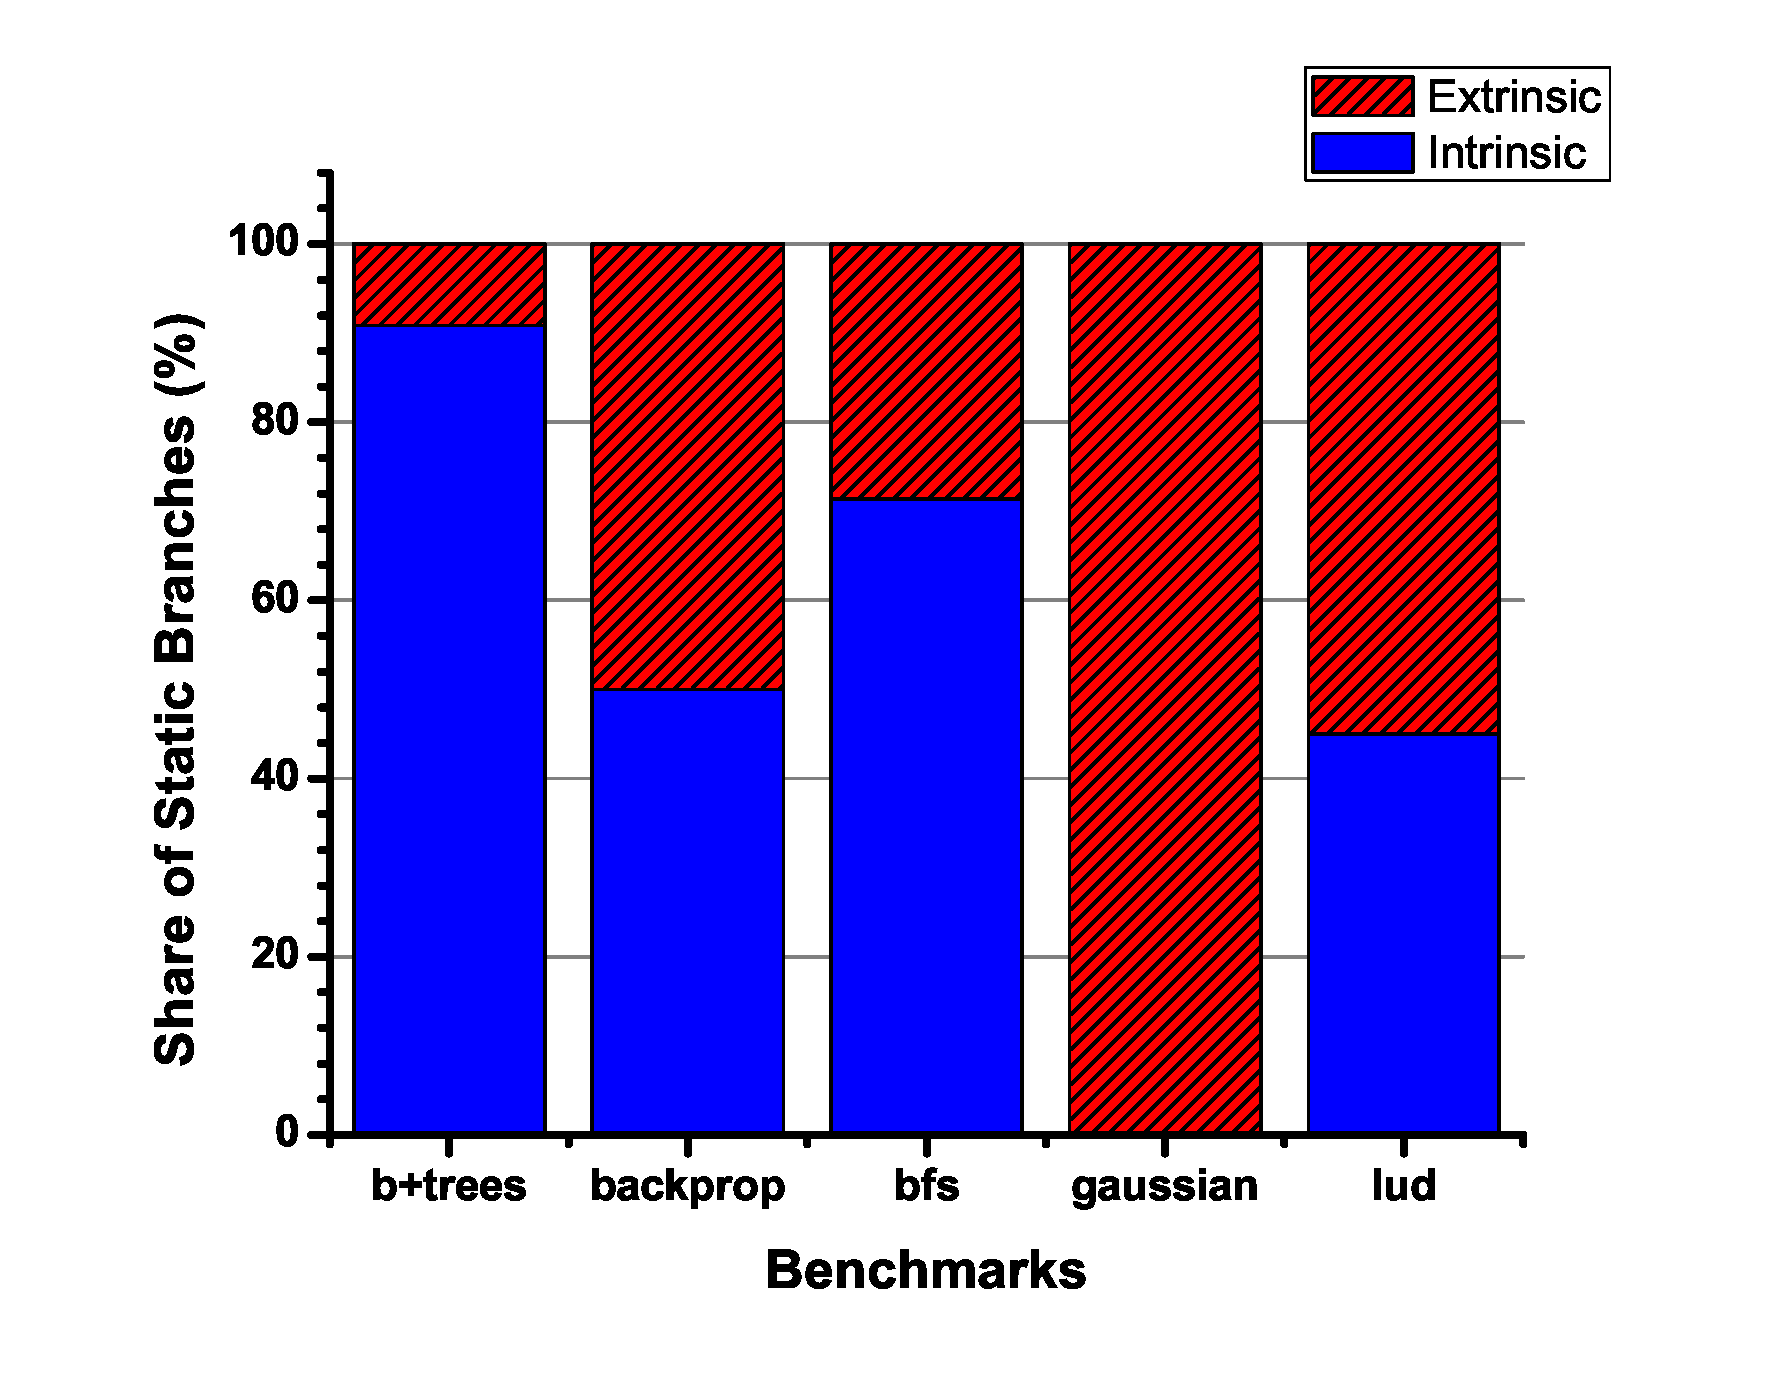
\includegraphics[width=10cm]{static-branches}
		\caption{static count for branch instructions
			\label{fig:static-branches}}
	\end{subfigure}
	\begin{subfigure}{0.45\textwidth}
		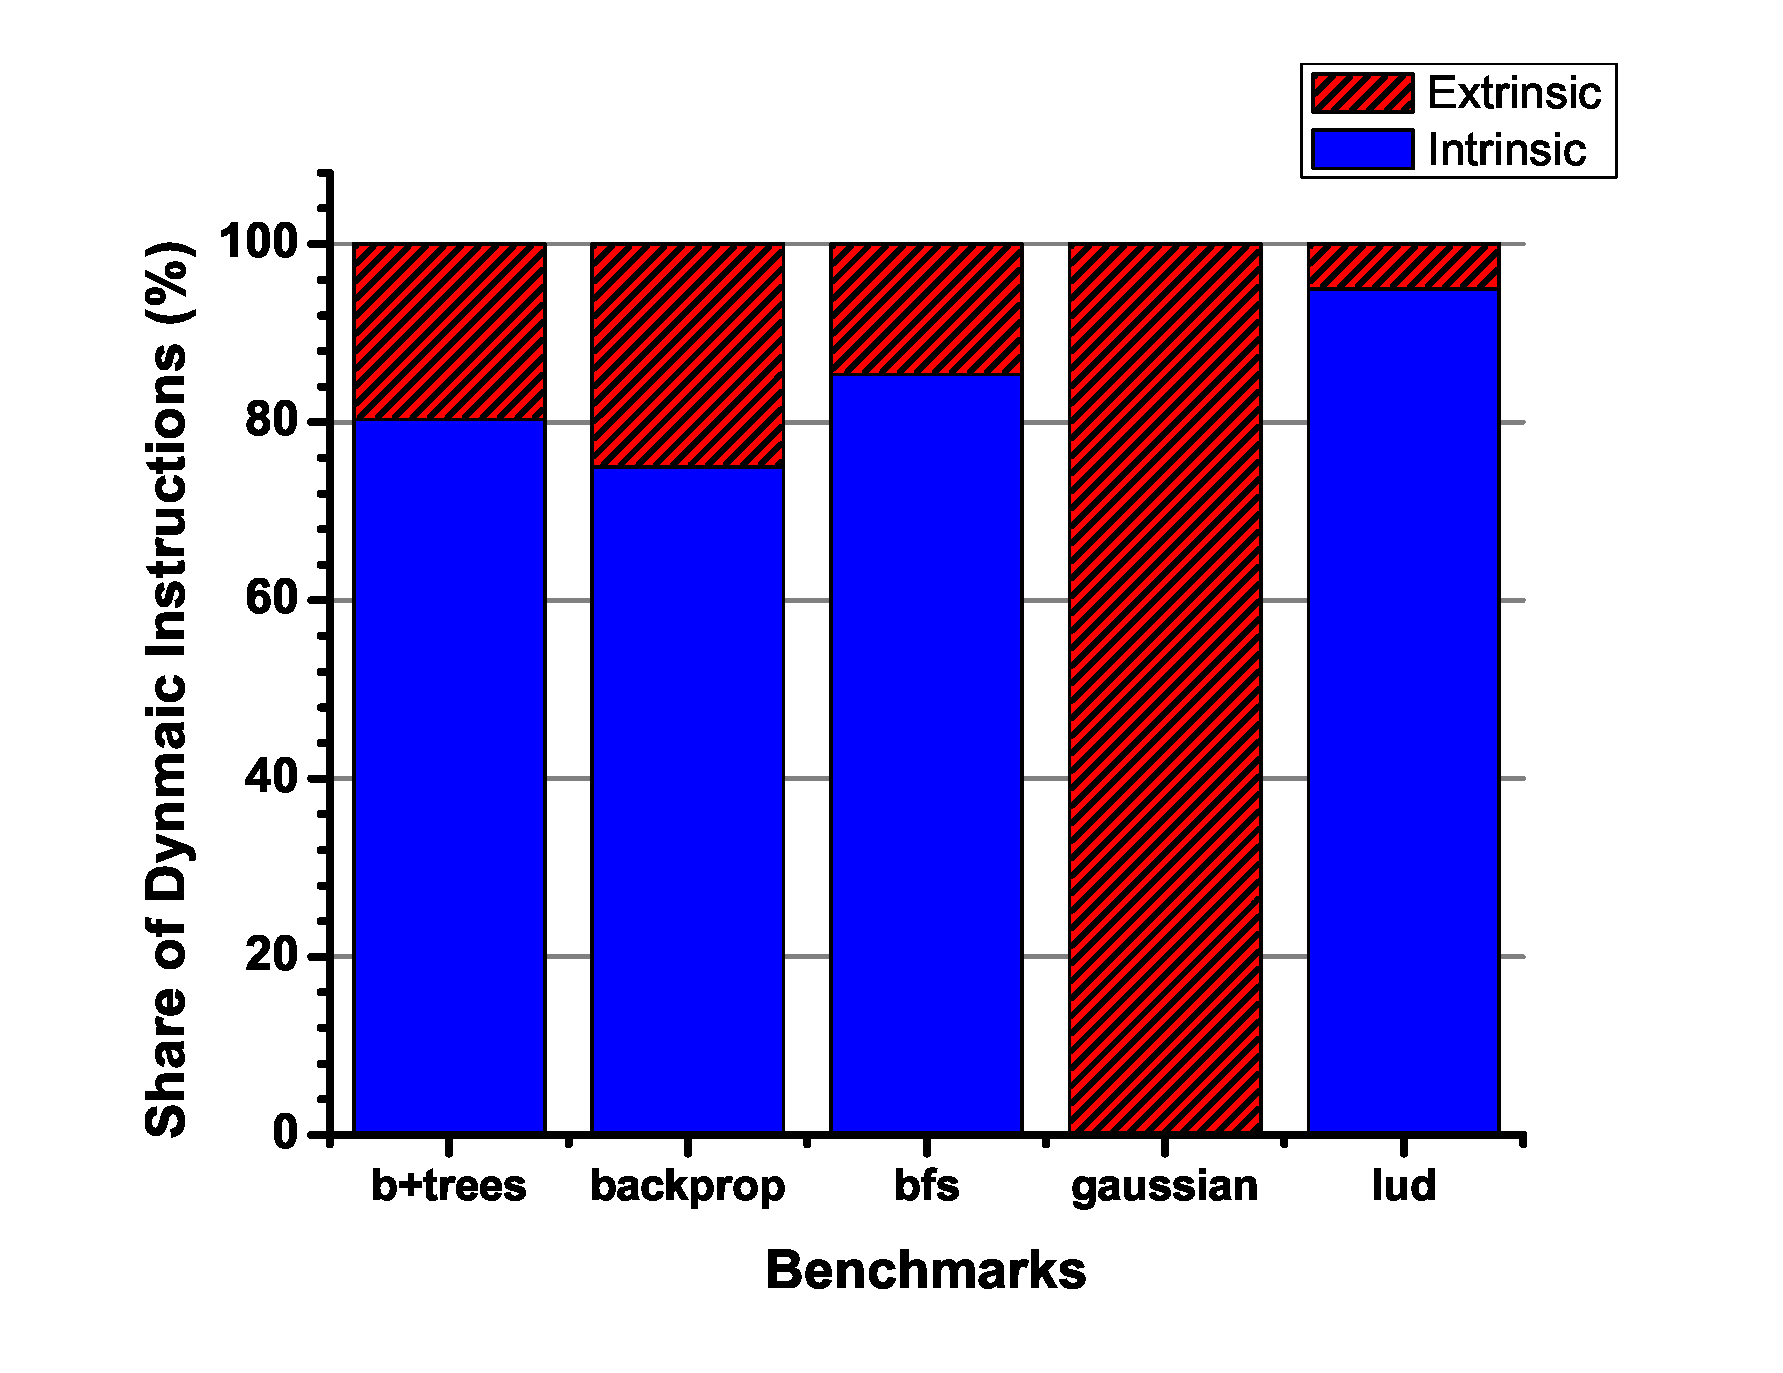
\includegraphics[width=10cm]{dynamic-branches}
		\caption{dynamic count for branch instructions
			\label{fig:dynamic-branches}}
	\end{subfigure}
	\caption{Distribution of the number of branches encountered in different benchmarks
		\label{fig:static-dynamic-distribution-plot}}
\end{figure*}
	Figure \ref{fig:static-dynamic-distribution-plot} shows the distribution of intrinsic and extrinsic branch instructions in terms of their static and dynamic counts. Static counts are measured by analyzing the compiled PTX code, whereas, the dynamic count is obtained from the branch target buffer shown in Figure \ref{fig:btb-example}.

\subsection{Performance impact}
\begin{figure}
	\centering
	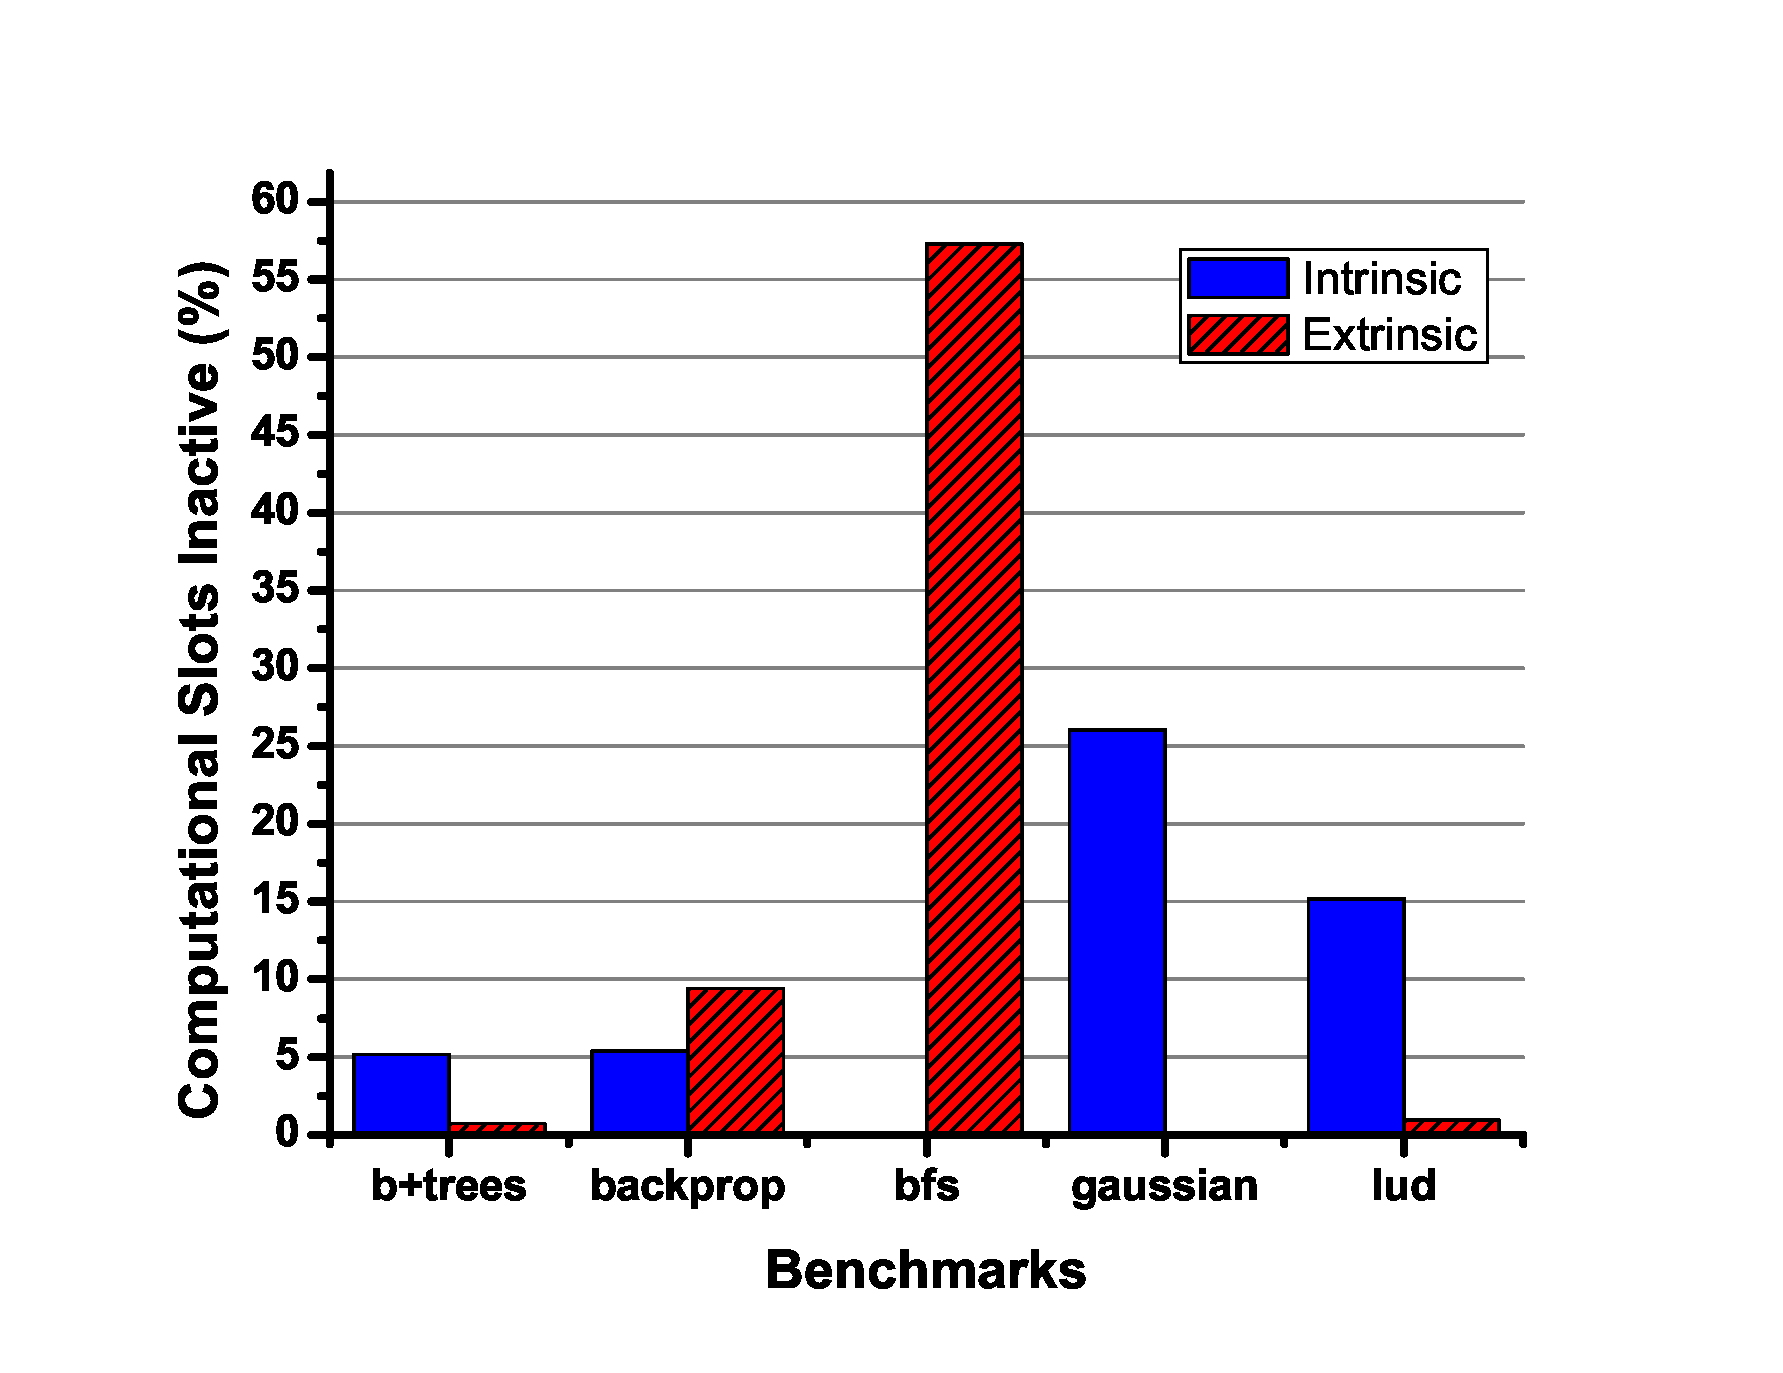
\includegraphics[width=10cm]{computational-slots-wasted}
	\caption{Percentage of computational slots wasted by the two categories of branch instructions
		\label{fig:computational-slots-wasted}}
\end{figure}
As described in Sections \ref{sec:problem-description} and \ref{sec:our-approach}, for each PTX instruction, we measure the total number of slots that were 1. Active, 2. Inactive due to an intrinsic branch and 3. Inactive due to an extrinsic branch. Finally, for any benchmark, we evaluate the aggregate of these metrics over the entire period of time when the benchmark was running. In Figure \ref{fig:computational-slots-wasted}, we report the fraction of total available slots that were wasted due to intrinsic and extrinsic branches respectively.

\subsection{Branch characteristics}
\begin{figure}
	\centering
	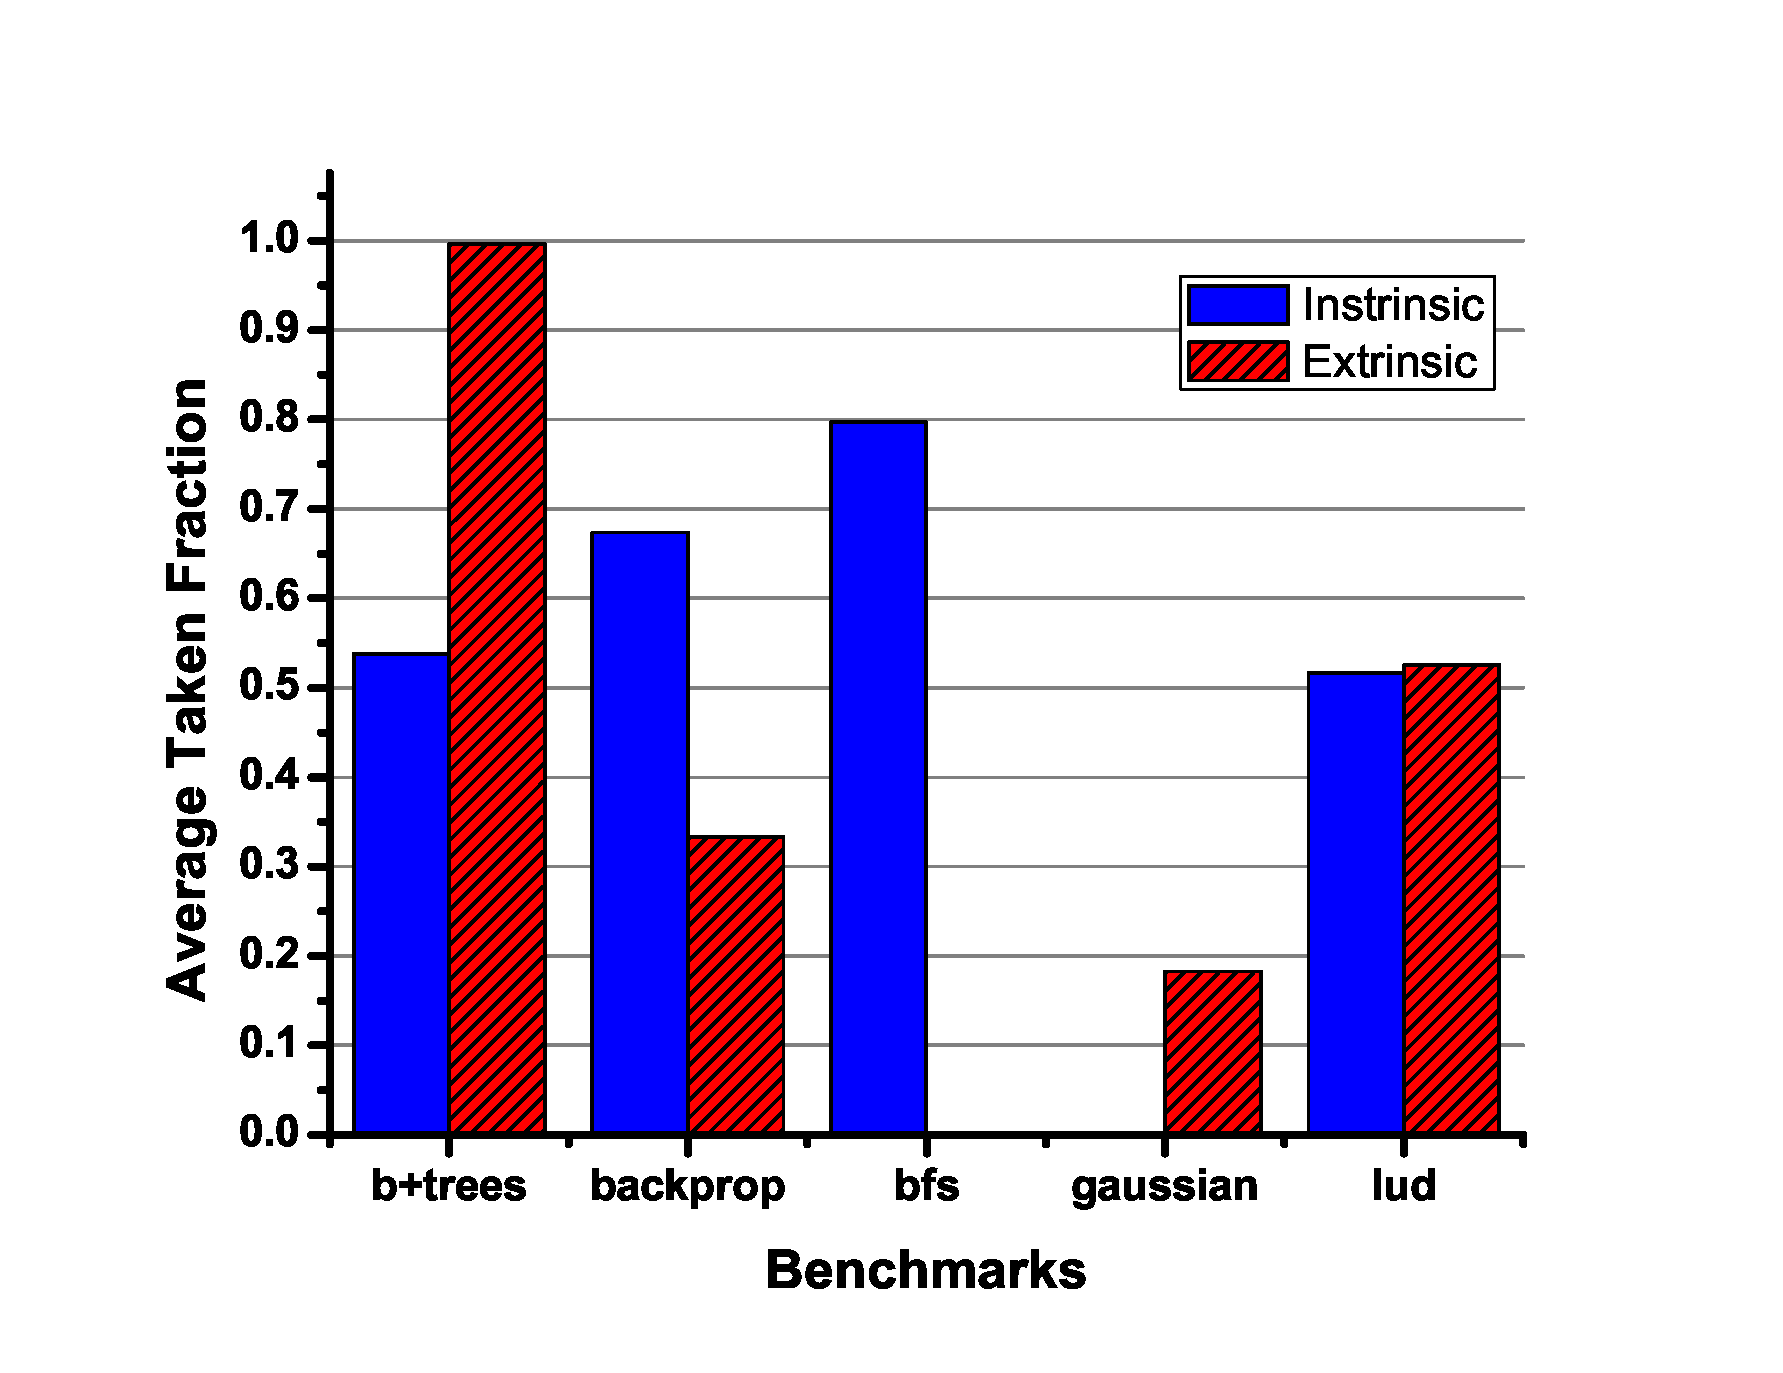
\includegraphics[width=10cm]{taken-fraction}
	\caption{Characterizing extrinsic and intrinsic branches based on the fraction of times they are taken when encountered
		\label{fig:taken-fraction}}
\end{figure}
In Figure \ref{fig:taken-fraction}, we report the weighted average of taken fractions (normalized by the instances for each branch, as reported in Figure \ref{fig:btb-example}) for each class of branches.




% An example of a floating figure using the graphicx package.
% Note that \label must occur AFTER (or within) \caption.
% For figures, \caption should occur after the \includegraphics.
% Note that IEEEtran v1.7 and later has special internal code that
% is designed to preserve the operation of \label within \caption
% even when the captionsoff option is in effect. However, because
% of issues like this, it may be the safest practice to put all your
% \label just after \caption rather than within \caption{}.
%
% Reminder: the "draftcls" or "draftclsnofoot", not "draft", class
% option should be used if it is desired that the figures are to be
% displayed while in draft mode.
%
%\begin{figure}[!t]
%\centering
%\includegraphics[width=2.5in]{myfigure}
% where an .eps filename suffix will be assumed under latex, 
% and a .pdf suffix will be assumed for pdflatex; or what has been declared
% via \DeclareGraphicsExtensions.
%\caption{Simulation results for the network.}
%\label{fig_sim}
%\end{figure}

% Note that the IEEE typically puts floats only at the top, even when this
% results in a large percentage of a column being occupied by floats.

%\begin{table}[!t]
%% increase table row spacing, adjust to taste
%\renewcommand{\arraystretch}{1.3}
% if using array.sty, it might be a good idea to tweak the value of
% \extrarowheight as needed to properly center the text within the cells
%\caption{An Example of a Table}
%\end{table}

\section{Discussion}

%----------------------------------------------------------------------------------------
%	DISCUSSION
%----------------------------------------------------------------------------------------

\label{sec:discussion}
\par{Static versus Dynamic Branches: The figures \ref{fig:static-branches} and \ref{fig:dynamic-branches} demonstrate that the benchmarks we have
tested tend to have more share of Instrinsic branches in their Dynamic branch counts than their Static counterpart. The share of intrinsic branches rises the most for \textsl{lud}: from less than 50\% to above 95\%. \textsl{lud}'s LU Decomposition algorithm has a loop which executes all the intrinsic branches in successive iteration. Most of the extrinsic branches only execute once and are involved in initializations or intermediate data movement and setup. Hence, we see a dramatic improvement in the share of intrinsic branches for \textsl{lud}. \textsl{backprop} and \textsl{bfs} also have a similar behaviour, perhaps largely due to their iterative nature even in a data-parallel GPU code. \textsl{b+trees}, however, sees a reduction of share of intrinsic branches. This is perhaps due to the repeated data-bound checks that it must do while pointer-chasing down the tree. Finally, \textsl{gaussian} has no intrinsic branches, a feature unique to it as most branches in its code are data-bound checks while performing scalar product. With the exception of \textsl{gaussian} (The Gaussian Elimination algorithm), it seems that a task which is iterative and has loops in its main Kernel code may have a higher share of intinsic branches to its dynamic branch count. This may suggest that most intrinsic branches are in the critical, repetitive body of the code which is a reasonable expectation.}

\par{Share of Computational Slots Inactive: The results for this metric \ref{fig:computational-slots-wasted} does not demonstrate a clear distinction between the static and dynamic branches. Although there is insufficient data to deny existence of any distinct behaviour between the two types, it seems almost certain that extrinsic branches seem to have a significant share in the Inactive slots. For instance, three of the five tested (\textsl{gaussian}, \textsl{lud} and \textsl{backprop}) have a larger share of inactivity due to their extrinsic branches. It is especially perplexing for \textsl{lud}, where although most dynamic branches are overwhelmingly intrinsic (\ref{fig:dynamic-branches}) they contribute to little or nothing to Inactivity. Moreover, \textsl{bfs} wastes more than half of its slots available on inactive intrinsic branches. In any case, we think the data here is too small to discern a general trend, but maybe sufficient to proceed with further investigation on the share of inactivity due to extrinsic branches.
}

\par{Taken Fraction: The results of taken fraction (Figure \ref{fig:taken-fraction}) are also in-conclusive. This is the metric which clearly demonstrates that more data will be needed, as no distinct extrinsic branch behaviour is visible as was expected. Although \textsl{b+trees} have always taken extrinsic branches, and \textsl{bfs} has none; \textsl{backprop}, \textsl{lud} and \textsl{gaussian} have extrinsic taken fractions quite close to 0.5. Hence, much more work can be done in this direction in the future.
}


\section{Conclusion}

%----------------------------------------------------------------------------------------
%	COLCLUSION
%----------------------------------------------------------------------------------------

\label{sec:conclusion}
\par{Static versus Dynamic Branches: The figures \ref{fig:static-branches} and \ref{fig:dynamic-branches} demonstrate that the benchmarks we have
tested tend to have more share of Instrinsic branches in their Dynamic branch counts than their Static counterpart. The share of intrinsic branches rises the most for \textsl{lud}: from less than 50\% to above 95\%. \textsl{lud}'s LU Decomposition algorithm has a loop which executes all the intrinsic branches in successive iteration. Most of the extrinsic branches only execute once and are involved in initlziations or intermediate data movement and setup. Hence, we see a dramatic improvement in the share of intrinsic branches for \textsl{lud}. \textsl{backprop} and \textsl{bfs} also have a similar behaviour, perhaps largely due to their iterative nature even in a data-parallel GPU code. \textsl{b+trees}, however, sees a reduction of share of intrinsic branches. This is perhaps due to the repeated data-bound checks that it must do while pointer-chasing down the tree. Finally, \textsl{gaussian} has no intrinsic branches, a feature unique to it as most branches in its code are data-bound checks while performing scalar product. With the exception of \textsl{gaussian} (The Gaussian Elimination algorithm), it seems that a task which is iterative and has loops in its main Kernel code may have a higher share of intinsic branches to its dynamic branch count. This may suggest that most intrinsic branches are in the critical, repetitive body of the code which is a reasonable expectation.}

\par{Share of Computational Slots Inactive: The results for this metric \ref{fig:comp-slots-wasted} does not demonstrate a clear distinction between the static and dynamic branches. Although there is insufficient data to deny existence of any distinct behaviour between the two types, it seems almost certain that extrinsic branches seem to have a significant share in the Inactive slots. For instance, three of the five tested (\testsl{gaussian}, \textsl{lud} and \textsl{backprop}) have a larger share of inactivity due to their extrinsic branches. It is especially perplexing for \textsl{lud}, where although most dynamic branches are overwhelmingly intrinsic (\ref{fig:dynamic-branches}) they contribute to little or no contribution to Inactivity. Moreover, \textsl{bfs} wastes more than half of its slots available on inactive intrinsic branches. In any case, we think the data here is too small to discern a general trend, but maybe suffiecient to undertake further investigation on the extent of damage by extrinsic branches.
}

\par{Taken Fraction: The results of taken fraction (\ref{fig:taken-fraction} are also in-conclusive. This is the metric which clearly demonstrates that more data will be needed. 
	However, this gain in performance is one side of a trade off. Since GPUs were originally designed to perform graphics manipulations, which are inherently data parallel, the performance of similar applications on a GPU results in significantly better performance as compared to a CPU. The flip side of the trade off is the loss of generality. General purpose CPUs are equipped with accurate branch prediction, Out of Order (OoO) cores, multi-level caches etc. in order to extract the maximum possible amount of instruction level parallelism (ILP) and to mitigate the performance hit that might arise from complicated control flow or poor spatial locality of data in the programs. On a GPU operating on a similar power/energy budget, these resources are reallocated to provide several, but extremely simple (almost bare) pipelines. This is done, assuming that the programs that run on this machine will exhibit a staggering amount of data parallelism.
}



% conference papers do not normally have an appendix


% use section* for acknowledgment
\section*{Acknowledgment}


The authors would like to thank...

% trigger a \newpage just before the given reference
% number - used to balance the columns on the last page
% adjust value as needed - may need to be readjusted if
% the document is modified later
%\IEEEtriggeratref{8}
% The "triggered" command can be changed if desired:
%\IEEEtriggercmd{\enlargethispage{-5in}}

\begin{thebibliography}{1}

\bibitem{IEEEhowto:kopka}
H.~Kopka and P.~W. Daly, \emph{A Guide to \LaTeX}, 3rd~ed.\hskip 1em plus
  0.5em minus 0.4em\relax Harlow, England: Addison-Wesley, 1999.

\end{thebibliography}

\end{document}


